% ============================================================
% IEEE Transactions (Q1) formati - IEEEtran sinifi, iki sutun.
% Overleaf'te veya texlive-full ile derlenir (IEEEtran standarttir).
% Turkce karakterler utf8 + T1 + lmodern ile calisir.
% ============================================================
\documentclass[10pt,journal]{IEEEtran}

\usepackage[utf8]{inputenc}
\usepackage[T1]{fontenc}
\usepackage{lmodern}
\usepackage{amsmath,amssymb}
\usepackage{booktabs}
\usepackage{graphicx}
\usepackage{cite}
\usepackage[hidelinks]{hyperref}

\begin{document}

\title{Transformer İleri-Besleme Katmanlarında Yapılandırılmış Seyreklik:\\
Kapsama, Derinlik ve Dağıtık İletişim Ödünleşiminin\\ Kontrollü Bir İncelemesi}

\author{Mustafa Selman Durmaz%
\thanks{Yazar, TÜBİTAK ULAKBİM TRUBA/ARF Eğitim Projesi kapsamında çalışmıştır
(proje kodu \texttt{egitimg35}). E-posta: dselman1134@gmail.com.}%
\thanks{Bu araştırmada yer alan tüm nümerik hesaplamalar TÜBİTAK ULAKBİM, Yüksek
Başarım ve Grid Hesaplama Merkezi'nde (TRUBA kaynaklarında) gerçekleştirilmiştir.}}

\markboth{TÜBİTAK ULAKBİM TRUBA/ARF Eğitim Projesi, Ağustos 2026}%
{Durmaz: Transformer FFN Katmanlarında Yapılandırılmış Seyreklik}

\maketitle

\begin{abstract}
Büyük dil modellerinde ileri-besleme (FFN) katmanları parametrelerin ve hesap yükünün büyük
bölümünü barındıran, iki yoğun dikdörtgen ağırlık matrisinden oluşan bileşenlerdir. Bu
matrislerin \emph{yoğun} olması bir zorunluluk mu yoksa gevşetilebilir bir varsayım mı
sorusunu, \emph{eşit parametre ve eşit FLOP} kısıtı altında yedi farklı bağlantı deseni
(yoğun, halka, küçük-dünya, rastgele, blok-köşegen, mozaik, kelebek) üzerinde kontrollü
olarak inceliyoruz. Deneyleri sekiz adet NVIDIA H200 hızlandırıcı üzerinde üç ölçekte
(katman, mimari, dağıtık) yürütüyoruz; toplam 326 eğitim koşusu, çoklu rastgele tohum ve
anlamlılık testleriyle raporlanıyor. Dört ana bulgu elde ediyoruz. Birincisi, aynı yoğunlukta
model kalitesini belirleyen şeyin desenin \emph{adı} olmadığını; ancak katman başına
\emph{kapsamanın} da tek başına yetmediğini gösteriyoruz: kapsaması özdeş iki desen arasında
$9.6\sigma$ fark ölçülebilmektedir. Bunun yerine \emph{karışma derinliğini} ($\tau$: her
çıktının her girdiye erişmesi için gereken katman sayısı) tanımlıyoruz; $\tau$ eşitse desenler
ayırt edilemez ($\sigma\le0.95$), $\tau\le L$ ile $\tau>L$ arasındaki sınır ise her yoğunlukta
anlamlıdır. $\tau$'yu önceden kaydedilmiş iki öngörüyle sınıyoruz: kelebeğin aşaması
dondurulduğunda kalitesinin bloğunkine düşmesi gerekir (ölçüm bu noktayı $0.14\sigma$
yakınlıkla tutturur), ve en seyrek rejimde kapsaması yarı kadar olan kelebeğin --- karışmasını
tamamlayabilen tek desen olduğu için --- halkayı geçmesi gerekir ($2.5\sigma$ ile geçer).
İkincisi, derinliğin etkisinin tek yönlü olmadığını, $\tau$ eşiğinde
açığın kapanıp ötesinde doygunlukla yeniden açıldığını ölçüyoruz. Üçüncüsü, kelebeğin halkaya
görünür üstünlüğünün öz-rehberli eğitim altında eridiğini ($12.0\sigma \to
1.5\sigma$) --- yani mimari sanılan farkın önemli bir bölümünün optimizasyon zorluğu olduğunu
--- gösteriyoruz. Dördüncüsü, dağıtık ortamda kelebek parçalamanın katman başına
muhatap sayısını $P{-}1$'den $1$'e düşürdüğünü fakat bu kazancın küçük ve ölçekle azalan bir
kalite bedeliyle geldiğini gösteriyoruz. Bu ödünleşimin bilgi-teorik bir sınıra dayandığını
(katman başına tam kapsama ile tek-muhatap iletişimin aynı katmanda bağdaşmadığını)
belirtiyor ve yöntemin hangi altyapı koşullarında rasyonel olduğunu bir karar modeliyle
nicelleştiriyoruz. Çalışmanın katkısı yeni bir yöntem değil, dağıtık FFN tasarımındaki
iletişim--kalite ödünleşiminin kontrollü bir haritasıdır.
\end{abstract}

\begin{IEEEkeywords}
Yapılandırılmış seyreklik, ileri-besleme ağı, dağıtık eğitim, tensor paralelliği, kelebek
matrisler, iletişim verimliliği, büyük dil modelleri.
\end{IEEEkeywords}

\IEEEpeerreviewmaketitle

% ============================================================
\section{Giriş}
% ============================================================
\IEEEPARstart{T}{ransformer} \cite{vaswani2017} tabanlı büyük dil modellerinde parametre
ölçeğinin artması,
başarımın temel belirleyicisi olmakla birlikte \cite{kaplan2020,chinchilla2022} bellek bant
genişliği ve hızlandırıcılar
arası iletişim sınırları nedeniyle bir altyapı darboğazı yaratmaktadır. Bir Transformer
katmanının parametrelerinin yaklaşık üçte ikisi ileri-besleme ağındadır (FFN); bu ağ, gizli
boyutu model boyutunun dört katına genişleten ($d \rightarrow 4d$) ve tekrar daraltan
($4d \rightarrow d$) iki \emph{yoğun} matristen oluşur. Parametre ve hesap yükünü azaltmak
amacıyla bu matrislerin düşük-ranklı, blok-köşegen, kelebek veya genel seyrek biçimlerle
değiştirilmesi geniş bir araştırma alanı oluşturmuştur.

Bu literatür iki ayrı eksende ilerlemiştir. Birinci eksen \emph{tek cihaz verimliliğine}
odaklanır: yapılandırılmış matrisler parametre ve teorik işlem sayısını düşürür, ancak
kalite ve gerçek hız üzerindeki etkileri kullanılan uygulamaya bağlıdır. İkinci eksen
\emph{dağıtık iletişime} odaklanır: model tek bir hızlandırıcıya sığmadığında Tensor
Paralelliği (TP) gibi teknikler zorunlu hale gelir ve bu teknikler her katmanda cihazlar
arası \emph{all-reduce} kolektif iletişimi gerektirir. Bu iki eksen literatürde çoğunlukla
birbirinden bağımsız incelenmiştir.

Bu çalışmada iki ekseni tek bir kontrollü çerçevede birleştiriyor ve şu soruyu soruyoruz:
yoğun FFN matrisi varsayımını terk etmek, parametre ve işlem sayısı sabit tutulduğunda,
kaliteyi, hızı ve dağıtık iletişim yükünü nasıl etkiler? Sorunun kritik yanı ``eşit parametre
ve eşit FLOP'' kısıtıdır: parametre sayısını düşüren bir karşılaştırma, farkın seyrek modelin
\emph{daha küçük} olmasından mı yoksa \emph{yapısından} mı kaynaklandığını belirsiz bırakır.
Biz gizli katmanı genişletip yoğunluğu düşürerek tüm varyantların parametre ve işlem sayısını
eşitliyoruz; böylece değişen tek etken ağırlık matrisinin \emph{şekli} olur.

\emph{Motivasyon.} Çalışmanın başlangıç motivasyonu, coğrafi olarak dağınık hesaplama
kaynaklarını tek bir model eğitiminde birleştirme senaryosuydu. Bu senaryoda darboğaz toplam
işlem gücü değil, düğümler arasındaki dar iletişim hattıdır. Bir FFN'in ağırlık matrisi yerel
bir bağlantı yapısına sahipse, o matris parçalandığında her parçanın yalnızca birkaç komşuyla
haberleşmesi yeterli olabilir; bu da her katmanda tüm düğümlerin haberleştiği yoğun TP'nin
aksine dar hatlarda çalışabilme umudu doğurur. Bu çalışma bu umudu doğrudan ve niceliksel
biçimde sınamaktadır.

\emph{Çalışmanın niteliği.} Bu bir yöntem-öneri çalışması değil, bir kontrollü ampirik
karakterizasyon çalışmasıdır. Amacımız yeni bir mimarinin üstünlüğünü ilan etmek değil;
hangi koşulda hangi tasarım tercihinin ne kazandırıp ne kaybettirdiğini, kontrol gruplarıyla
ve istatistiksel anlamlılıkla ölçmektir. Sonuçlarımızın önemli bir kısmı olumsuz veya
nüanslıdır ve bu tür sonuçların dürüstçe raporlanmasını çalışmanın temel değeri sayıyoruz.

Katkılarımız şunlardır: (1) Eşit parametre/FLOP kısıtı altında yedi FFN topolojisini
karşılaştırıyor, katman başına kapsamanın kaliteyi açıklamakta yetersiz kaldığını gösteriyor
ve yerine \emph{karışma derinliği} $\tau$'yu öneriyoruz; $\tau$'yu önceden kaydedilmiş,
çürütülebilir bir nokta öngörüsüyle sınıyoruz. (2) Derinliğin etkisinin $\tau$ eşiğine göre
yön değiştirdiğini --- eşiğe kadar eksik karışma, eşikten sonra doygunluk --- ölçüyor ve
``yapısız rastgele en iyidir'' bulgusunun bu ikinci mekanizmanın eseri \emph{olmadığını} bir
sabit-maske kontrolüyle ayrıştırıyoruz. (3) Sekiz H200 üzerinde, rank başına eşit
parametreyle, kelebek parçalamanın muhatap sayısını $P{-}1$'den $1$'e ve FFN iletişimini
$\sim\!7\times$ düşürdüğünü, fakat dikkat all-reduce'u nedeniyle uçtan uca kazancın
$\sim\!2\times$ ile sınırlı olduğunu ölçüyoruz. (4) Katman başına tam kapsama ile tek-muhatap
iletişimin bağdaşmadığı bir bilgi-teorik sınır belirtiyoruz. (5) Yöntemin rasyonel olduğu
koşul aralığını bir karar modeliyle nicelleştiriyoruz.

% ============================================================
\section{İlgili Çalışmalar}
% ============================================================
\emph{Paralellik yığını.} Büyük modelleri eğitmek için kullanılan paralellik biçimleri
birbirini tamamlar: veri paralelliği bellek yükünü optimizatör durumlarını parçalayarak azaltır
(ZeRO \cite{zero2020}, FSDP \cite{fsdp2023}), ardışık düzen paralelliği katmanları cihazlara
böler \cite{gpipe2019}, tensör paralelliği ise tek bir katmanı böler ve her katmanda
all-reduce gerektirir \cite{megatron2019,narayanan2021}. Bu çalışmanın konusu son gruptur:
FFN'in tensör paralelliğindeki iletişim yükünü, ağırlık matrisinin \emph{şeklini} değiştirerek
azaltmanın mümkün olup olmadığı. Etkinleştirme belleği ve dizi paralelliği üzerine çalışmalar
\cite{korthikanti2023} ile dikkat katmanını parçalayan yaklaşımlar \cite{ringattn2023} bu
eksene diktir.

\emph{Seyreklik biçimleri.} Ağırlık seyrekliği literatürü uzundur: büyüklüğe göre budama
\cite{han2015}, piyango bileti hipotezi \cite{frankle2019}, eğitim sırasında bağlantıları
yeniden dağıtan yöntemler \cite{rigl2020} ve tek seferde budama \cite{sparsegpt2023}.
Donanım tarafında NVIDIA'nın 2:4 yapılandırılmış seyrekliği \cite{nm2021} bir desenin
hızlanmaya dönüşmesi için ne kadar dar bir yapı gerektiğini gösterir. Graf teorisinden
esinlenen genişleteç (expander) ağları \cite{expander2018}, bizim ``kapsama'' sezgimize
yakın bir motivasyonla seyrek katmanları bağlantılılık üzerinden tasarlar. Kelebek
çarpanlamaları önce hızlı dönüşümleri öğrenmek için kullanılmış \cite{dao2019}, sonra
seyrek eğitim için genelleştirilmiştir \cite{pixelbutterfly2022}.

\emph{Yapılandırılmış FFN matrisleri.} Yoğun FFN matrislerini düşük-ranklı, blok veya kelebek
biçimlerle değiştirme çalışmaları parametre ve işlem sayısını düşürmeyi hedefler. Wei ve
arkadaşları \cite{wei2024} düşük-ranklı FFN'lerin sıfırdan eğitiminde optimizasyon
kararsızlıklarını gözlemlemiş ve eğitimin başında geçici bir yoğun dal kullanan öz-rehberli
eğitim yöntemini önermiştir. Dao ve arkadaşlarının Monarch matrisleri \cite{dao2022} iki
blok-köşegen matrisin permütasyonla çarpımıdır ve toplu matris çarpımı (bmm) çekirdeklerinden
yararlanarak yoğun çarpıma göre $2\times$'e varan hızlanma sağlar. Bu çalışmalar tek cihaz
verimliliğine odaklanır.

\emph{Dinamik seyreklik: uzman karışımları.} FFN'i seyrekleştirmenin alanda fiilen benimsenmiş
yolu, uzman karışımlarıdır (MoE): her belirteç bir yönlendirici tarafından birkaç uzmana
gönderilir \cite{shazeer2017,gshard2021,switch2022}. Bu, bizim incelediğimizden farklı bir
seyreklik türüdür.
MoE'de seyreklik \emph{girdiye bağlı ve dinamiktir}; ağırlık matrisinin kendisi yoğun kalır,
seyrek olan uzman seçimidir. Dağıtık maliyeti de farklıdır: uzman paralelliği her katmanda
bir \emph{all-to-all} gerektirir; bu kolektif, incelediğimiz sabit-muhatap değiş-tokuşundan
dar hatlarda daha pahalıdır. Bu çalışmanın konusu ise \emph{statik yapısal} seyrekliktir:
desen eğitimden önce bellidir, muhatap kümesi sabittir ve yönlendirme maliyeti yoktur.
İki yaklaşım rakip değil diktir; MoE'nin kalite/verim dengesi bizim ölçtüğümüz
iletişim--kapsama ödünleşiminden bağımsızdır.

\emph{İletişimi optimizasyon tarafından azaltmak.} Başlangıç motivasyonumuz olan ``dar hat
üzerinden dağınık kaynakları birleştirme'' hedefine, ağırlık yapısını değiştirmeden de
saldırılmıştır: yerel-SGD ailesi \cite{stich2019} ve DiLoCo \cite{diloco2023} düğümleri her
adımda değil, yüzlerce adımda bir senkronize ederek iletişimi iki mertebe azaltır; SWARM
\cite{swarm2023} ve Petals \cite{petals2023} güvenilmez ve heterojen düğümler üzerinde
çalışmayı hedefler. Bu yaklaşımlar senkronizasyon
\emph{takvimini} değiştirir, matrisin şeklini değil. Bulgularımız bu literatürle çelişmez,
onu tamamlar: aynı hedefe ağırlık yapısı ekseninden gidildiğinde yolun bir bilgi-teorik
sınırla kapandığını gösteriyoruz (Bölüm~\ref{sec:sinir-teori}), ki bu da çözümün neden
optimizasyon ekseninde arandığını açıklar.

\emph{Desen çeşitliliği ve derinlik.} ShuffleSparse \cite{shufflesparse2025}, sabit
eksen-hizalı seyreklik desenlerinin derinlikle çarpanlı ifade gücü kazanamadığını, buna
karşılık derinlikle değişen tam-ranklı karıştırıcıların bu kapasiteyi kazandığını teorik
olarak göstermiştir. Bu çalışmada söz konusu teoriyi bağımsız ölçümle doğruluyoruz.

\emph{Dağıtık iletişim.} Tensor paralelliğinde her katman iki all-reduce gerektirir ve bu
iletişim çıkarım süresinin önemli bir bölümünü oluşturabilir \cite{flashcomm2024}.
Blok-köşegen yapılarla iletişimi azaltan yaklaşımlar (BD-LoRA \cite{bdlora2025},
DeTransformer \cite{detransformer2024}) sabit desenlere dayanır ve çoğunlukla çıkarım için
tasarlanmıştır. Bizim incelediğimiz eksen, derinlikle değişen bir deseni dağıtık parçalama
topolojisi olarak kullanmaktır; taramamızda ifade gücü ve muhatap sayısını birlikte ele alan
bir çalışmaya rastlamadık. Dikkat katmanındaki iletişimi azaltan yaklaşımlar (dizi
paralelliği, halka-dikkat) bu eksene diktir ve FFN tarafındaki kazançla birleştirilebilir;
ölçtüğümüz $\sim\!2\times$'lik uçtan uca tavan (Bölüm~\ref{sec:sinir}, madde 1) tam olarak bu
birleşimin yapılmamasından doğar.

% ============================================================
\section{Yöntem}
% ============================================================
\subsection{Eşit parametre ve eşit FLOP protokolü}
Standart bir FFN, gizli boyutu $4d$ olan yoğun bir aradır:
$\mathrm{FFN}(x) = W_{\downarrow}\,\sigma(W_{\uparrow}x)$, burada
$W_{\uparrow}\in\mathbb{R}^{4d\times d}$, $W_{\downarrow}\in\mathbb{R}^{d\times 4d}$ ve toplam
parametre $8d^2$'dir. Seyrek bir varyantı adil karşılaştırmak için gizli boyutu $M\!\cdot\!d$'ye
genişletir, yoğunluğu $4/M$'ye düşürür ve sıfır olmayan bağlantı sayısını (nnz) yoğun modelle
eşit tutarız:
\begin{equation}
h = M\,d, \qquad \text{yoğunluk} = \frac{4}{M}, \qquad \mathrm{nnz} = 8d^2 .
\end{equation}
Böylece $M=4$ yoğun modelin kendisidir, $M=8$ yoğunluk $1/2$, $M=16$ yoğunluk $1/4$ demektir.
Bu protokol altında tüm varyantlar aynı parametre ve aynı işlem sayısına sahiptir; değişen tek
şey ağırlık matrisinin şeklidir.

\subsection{Bağlantı desenleri}
Yedi FFN deseni karşılaştırıyoruz (Tablo~\ref{tab:varyant}). \emph{Rastgele} desen kritik bir
kontrol grubudur: bir farkın yapıdan mı yoksa yalnızca seyreklikten mi geldiğini ancak bu grup
ayırır. \emph{Mozaik} (satranç tahtası) görünüşte dağınık bir desendir ancak satır/sütun
permütasyonuyla blok-köşegene özdeştir. \emph{Kelebek}, katman $\ell$'de $r$ birimini
$r \oplus 2^{\ell}$ ile eşleyen, FFT tabanlı ve derinlikle değişen bir desendir.

\begin{table}[!t]
\centering
\footnotesize
\caption{FFN bağlantı desenleri ve ölçülen kapsama (yoğunluk $1/4$, $M{=}16$).}
\label{tab:varyant}
\begin{tabular}{@{}lll@{}}
\toprule
Desen & Tanım & Kapsama \\
\midrule
Yoğun          & tam bağlı, gizli $4d$          & 1.000 \\
Halka          & yerel poligon bandı            & 0.498 \\
Küçük-dünya    & bant $+$ birkaç uzun kenar     & 1.000 \\
Rastgele       & rastgele (kontrol grubu)       & 1.000 \\
Blok-köşegen   & bağımsız gruplar               & 0.250 \\
Mozaik         & satranç tahtası ($\equiv$ blok)& 0.250 \\
Kelebek        & FFT, derinlikle değişir        & 0.250 \\
\bottomrule
\end{tabular}
\end{table}

\subsection{Kapsama ölçüsü}
Bir FFN iki adımda bilgi karıştırır: $x \to h \to y$. Yukarı ve aşağı maskeleri
$U\in\{0,1\}^{h\times d}$, $D\in\{0,1\}^{d\times h}$ olmak üzere kapsamayı tanımlarız:
\begin{equation}
\label{eq:coverage}
\mathcal{C} = \frac{1}{d^2}\sum_{i,j}\mathbb{1}\!\left[(D\,U)_{ij} > 0\right],
\end{equation}
yani bir çıktı biriminin gizli katman üzerinden ulaşabildiği girdi birimlerinin ortalama
oranı. $\mathcal{C}=1$ tam karışım, düşük $\mathcal{C}$ bilginin yerel kaldığı anlamına gelir.
Kapsama ağırlık değerlerinden bağımsız, yalnızca yapısal bir özelliktir ve eğitim yapmadan
hesaplanabilir (Şekil~\ref{fig:kapsama}).

\begin{figure*}[!t]
\centering
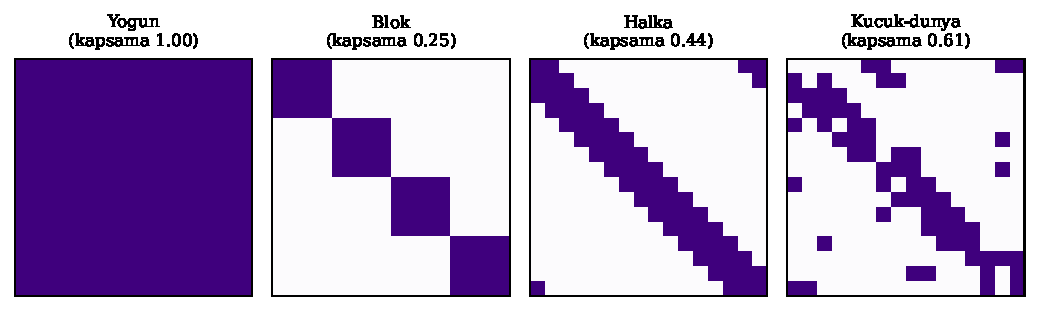
\includegraphics[width=0.92\textwidth]{fig_kapsama.pdf}
\caption{Kapsama kavramı. Dört bağlantı deseninin $16\times16$ ağırlık maskesi; mor hücreler
sıfır olmayan ağırlıklardır. Dört desende de satır başına aynı bağlantı sayısı (eşit parametre)
bulunur; değişen tek şey bu bağlantıların dağılımı, dolayısıyla kapsamadır.}
\label{fig:kapsama}
\end{figure*}

\subsection{Karışma derinliği}
\label{sec:tau}
Denklem~\eqref{eq:coverage} tek bir FFN'e bakar. Oysa bilgi yalnızca bir katmanda değil,
katmanlar boyunca da yayılır: $\ell$'inci katmanın erişim matrisi $R_\ell = D_\ell U_\ell$
olmak üzere $L$ katman sonundaki \emph{birikmiş kapsamayı} tanımlarız:
\begin{equation}
\label{eq:ceff}
\mathcal{C}_{\mathrm{eff}}(L) = \frac{1}{d^2}\sum_{i,j}
  \mathbb{1}\!\left[\left(R_L R_{L-1}\cdots R_1\right)_{ij} > 0\right],
\end{equation}
ve bundan \emph{karışma derinliğini} türetiriz:
\begin{equation}
\label{eq:tau}
\tau = \min\{\,L : \mathcal{C}_{\mathrm{eff}}(L) = 1\,\}.
\end{equation}
$\tau$, bir topolojinin her çıktının her girdiye erişebilmesi için kaç katman gerektirdiğini
söyler; $\mathcal{C}$ gibi ağırlıklardan bağımsızdır ve eğitim yapmadan, yalnızca maskeler
üzerinde ikili matris çarpımıyla hesaplanır. İki büyüklük farklı şeyler ölçer: blok-köşegen
bir maskenin bileşkesi yine blok-köşegendir, dolayısıyla blok için $\mathcal{C}_{\mathrm{eff}}$
her derinlikte sabit kalır ve $\tau$ tanımsızdır ($\tau>L$); buna karşılık kelebeğin aşaması
katmandan katmana döndüğü için $\tau = \lceil \log_2 d \rceil$ mertebesinde tamamlanır.
İkisinin katman başına kapsaması ($0.250$) aynı olduğu hâlde.

\emph{$\tau$ nasıl geliştirildi ve nasıl sınandı.} Sonuca bakarak ölçü uydurma (HARKing)
riskini açıkça ele alıyoruz. $\tau$'yu, kapsamanın başarısız olduğunu gördüğümüz $M{=}16$
ızgarası üzerinde formüle ettik. Ardından \emph{hiçbir değişiklik yapmadan} üç bağımsız veri
kümesine uyguladık: diğer yoğunluklar ($M \in \{8,32,64\}$), derinlik taraması
($L \in \{2,4,8,16\}$) ve dağıtık varyantlar. Son olarak, ölçünün değerini bir eğri uydurmayla
değil, \emph{çürütülebilir} iki öngörüyle sınadık; her ikisi de ilgili koşular
kuyruğa verilmeden önce deney betiklerine yazılarak kaydedilmiştir:

\begin{enumerate}
\item Kelebeğin aşaması tüm katmanlarda dondurulursa $\tau$'su $>L$'ye çıkar; kalitesi, aynı
katman içi kapsamaya sahip bloğun seviyesine \emph{düşmelidir}
(Bölüm~\ref{sec:sabit}).
\item $M{=}64$'te kapsama ile $\tau$ ters sıralama verir; ölçüm $\tau$'yu izlerse kelebek,
kapsaması iki katı olan halkayı \emph{geçmelidir} (Bölüm~\ref{sec:bulgu-tau}).
\end{enumerate}

Her iki öngörü de tutmuştur. Bu, $\tau$'nun veriye sonradan uydurulmuş bir tanım değil,
yanlışlanabilir bir hipotez olarak sınandığı anlamına gelir. Ölçünün başarısız olduğu tek
durumu da aynı disiplinle raporluyoruz.

\subsection{Uygulamalar ve kontroller}
Aynı matematiği iki biçimde hesaplarız: \emph{maskeli} (yoğun matmul $+$ ikili maske; kalite
deneyleri için, tüm varyantları aynı biçimde ele alır) ve \emph{bmm} (gerçek küçük matris
çarpımları; hız iddiaları için). Seyrek bir katmanın fan-in'i yoğun katmandan küçük olduğundan
tek bir başlangıç ölçeği tarafsız değildir; sonuçları üç başlangıç rejiminde (\texttt{gpt},
\texttt{kaiming}, \texttt{mixed}) ayrı ayrı raporlarız. Yapılandırılmış katmanların
optimizasyon zorluğunu incelemek için, eğitimin ilk \%30'unda FFN'e paralel geçici bir yoğun
dal ekleyen öz-rehberli eğitim rejimini \cite{wei2024} bir kontrol olarak uygularız.

\subsection{Modeller, veri ve istatistik}
Mimari taramasında karakter düzeyinde \texttt{text8} \cite{mahoney2011} üzerinde GPT-mini
($d{=}512$, 8 katman,
$\sim\!25$M) modelini 6000 adım eğitir, kaliteyi karakter başına bit (bpc) ile ölçeriz.
Ölçeklemede bayt düzeyinde \texttt{enwik9} üzerinde $d{=}1024$, 32 katman, $\sim\!403$M
parametreli bir modeli sekiz H200 üzerinde veri-paralel olarak $\sim\!2$B token ile eğitiriz.
Dağıtık ölçümü iki sunucu ($2{\times}4$ H200, InfiniBand) üzerinde yaparız. Tüm karşılaştırmalar
çoklu tohum üzerinden ortalama ve standart sapma ile raporlanır; iki ortalama farkının
anlamlılığını $\sigma = |\Delta| / \sqrt{\mathrm{SE}_1^2 + \mathrm{SE}_2^2}$ ile ölçer ve
$\sigma<2$ olan farkları gürültü sayarız.

% ============================================================
\section{Bulgular}
% ============================================================
\subsection{Kalite ve kapsama}
Tablo~\ref{tab:kalite} mimari taramasının sonuçlarını gösterir. Yoğunluk $1/2$'ye kadar
seyreklik istatistiksel olarak bedelsizdir ($\sigma \le 1.2$); yoğunluk $1/4$'e inince yoğun
model net kazanır ($+0.022$ bpc, $16\sigma$) ve fark yoğunluk düştükçe monoton artar. Aynı
yoğunluk içinde ise kaliteyi belirleyen şey desenin adı değildir: mozaik ile blok görünüşte
zıt olmalarına rağmen neredeyse aynı bpc'yi verir ($0.10\sigma$). Bu eşitliği veriden önce
öngörmüştük; ancak sonradan fark ettik ki mozaik, bloğun satır/sütun permütasyonudur ve
FFN gizli birimleri değiş-tokuş bakışımlı olduğundan iki varyant \emph{aynı model sınıfını}
tanımlar. Dolayısıyla bu eşitlik kapsama hipotezinin kanıtı değil, deney hattının ve tohum
gürültüsünün doğrulamasıdır; öyle raporluyoruz. Üçüncü gözlem, yapısız rastgele seyrekliğin
her yapılandırılmış desenden iyi olduğudur; küçük-dünya ile rastgele her yoğunlukta
istatistiksel olarak aynıdır. Bu bulgu ``düzenli topoloji rastgele seyreklikten iyidir''
beklentisini çürütür (yorumuna ilişkin bir çekince için Bölüm~\ref{sec:sinir}, madde 7).
Yoğunluk düştükçe desenlerin ayrışması Şekil~\ref{fig:yogunluk}'te görülür.

\subsection{Kapsama nerede yetmiyor: karışma derinliği}
\label{sec:bulgu-tau}
Katman başına kapsama $\mathcal{C}$ kaba sıralamayı verir, ama iki yönden de yanıltır.
$M{=}16$'da kelebek ile bloğun kapsaması \emph{aynıdır} ($0.250$) fakat aralarındaki fark
$0.0156$ bpc, yani $9.6\sigma$'dır; buna karşılık halka ile kelebeğin kapsaması \emph{iki
kat} farklıdır ($0.498$'e karşı $0.250$) ama ölçülen fark $0.0014$ bpc, yani $0.95\sigma$ ---
gürültü. Kapsama bu iki durumda da yanlış hüküm verir.

Denklem~\eqref{eq:tau}'daki karışma derinliği $\tau$ ikisini de düzeltir
(Tablo~\ref{tab:tau}). Belirleyici olan, karışmanın \emph{tamamlanıp tamamlanmadığıdır}:
$\tau \le L$ olan her desen ile $\tau > L$ olan her desen arasındaki fark her yoğunlukta
anlamlıdır (en zayıf ayrım $M{=}8$'de $2.03\sigma$, $M{=}16$'da $6.33\sigma$;
Şekil~\ref{fig:tau}). Bu sınırın
mekanizması yapısaldır: blok ve mozaiğin bileşkesi blok-köşegen kaldığı için
$\mathcal{C}_{\mathrm{eff}}$ derinlikten bağımsız olarak $0.25$'te takılı kalır, kelebek ise
aşaması döndüğü için üç katmanda $1.0$'a ulaşır. Tamamlayan desenler arasında kalite $\tau$
ile birlikte kötüleşir ve $\tau$'su eşit olanlar ayırt edilemez ($\sigma \le 0.95$); ancak
bu dereceli sıralamanın çözünürlüğü seyrekliğe bağlıdır: $M{=}16$'da $\tau{=}1$ ile
$\tau{=}3$ arası ayrışırken ($2.96\sigma$), $M{=}8$'de $\tau{=}1$ ile $\tau{=}2$ arası
gürültünün altında kalır ($0.02\sigma$). Yani $\tau$ sıralayıcı bir ölçüdür, metrik değil.

\emph{Bağımsız tekrar.} ``Aynı kapsama, farklı kalite'' karşıörneği tek bir yoğunluğa özgü
değildir: $M{=}32$'de kelebek ve blok yine aynı kapsamayı ($0.125$) paylaşır ve $7.1\sigma$
ayrışır, $M{=}64$'te aynı kapsamada ($0.062$) $9.0\sigma$ ayrışır. Üç yoğunlukta da ayıran
şey $\tau$'dur.

\emph{İki ölçünün ters hüküm verdiği durum.} $M{=}64$, kapsama ile $\tau$'nun yalnızca
büyüklükte değil \emph{sırada} çeliştiği bir hücre sunar. Orada halkanın katman başına
kapsaması ($0.123$) kelebeğinkinin ($0.062$) iki katıdır, dolayısıyla kapsama halkayı önde
sayar. Ancak halka sekiz katmanda karışmasını bitiremez
($\mathcal{C}_{\mathrm{eff}}{=}0.971$, $\tau>L$), kelebek bitirir ($\tau{=}5$); $\tau$ ters
yönde, kelebeği önde sayar. Ölçüm $\tau$'yu doğrular: kelebek $1.5544$, halka $1.5606$
($2.53\sigma$). Yarı kapsamalı desen, karışmasını tamamlayabildiği için kazanır. Bu öngörüyü
koşulardan önce kaydettik.

\emph{$\tau$'nun tek başarısızlığı.} Dört yoğunluk boyunca 41 ikili karşılaştırmanın
35'i doğru, 9'u istatistiksel olarak ayırt edilemez ve \emph{biri} ihlaldir. Sıralama hiçbir
yerde tersine dönmez; tek kusur bir ayırt-etme başarısızlığıdır: $M{=}64$'te rastgele ile
küçük-dünyanın ikisi de $\tau{=}1$ olduğu hâlde $8.2\sigma$ ayrışırlar. Bu beklenen bir
sınırdır --- $\tau$ ikili bir erişilebilirlik ölçüsüdür, erişimin \emph{dağılımını} görmez;
satır başına yalnızca 32 bağlantı kaldığında (bu yoğunlukta) ``her girdiye ulaşıyor'' ifadesi
kaliteyi belirlemek için fazla kabadır.

\begin{table}[!t]
\centering
\footnotesize
\caption{Karışma derinliği $\tau$, katman başına kapsamanın açıklayamadığı farkları açıklar
($M{=}16$, $L{=}8$). Kelebek ile blok aynı $\mathcal{C}$'ye sahiptir ama farklı $\tau$'ya;
halka ile kelebek farklı $\mathcal{C}$'ye sahiptir ama aynı $\tau$'ya. Ölçüm $\tau$'yu
izler: $\tau$'su eşit olan desenler ayırt edilemez, farklı olanlar anlamlıdır.}
\label{tab:tau}
\begin{tabular}{@{}lccccc@{}}
\toprule
Desen & Katmanlar arası & $\mathcal{C}$ & $\tau$ & val bpc & $n$ \\
\midrule
Rastgele    & değişken & 1.000 & 1     & $1.4691 \pm 0.0023$ & 9 \\
Küçük-dünya & değişken & 1.000 & 1     & $1.4696 \pm 0.0036$ & 6 \\
\midrule
Halka       & sabit    & 0.498 & 3     & $1.4752 \pm 0.0029$ & 6 \\
Kelebek     & değişken & 0.250 & 3     & $1.4766 \pm 0.0023$ & 6 \\
\midrule
Blok        & sabit    & 0.250 & $>L$  & $1.4923 \pm 0.0023$ & 3 \\
Mozaik      & sabit    & 0.250 & $>L$  & $1.4925 \pm 0.0040$ & 3 \\
\bottomrule
\end{tabular}
\end{table}

\begin{figure}[!t]
\centering
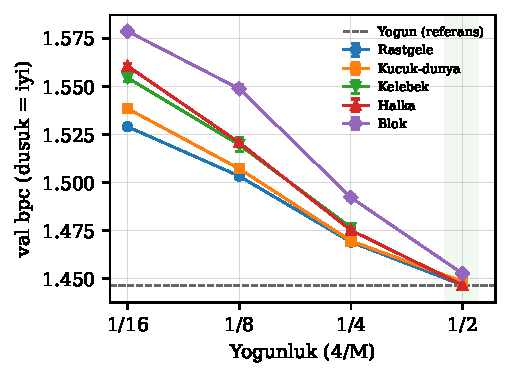
\includegraphics[width=0.95\columnwidth]{fig_yogunluk.pdf}
\caption{Yoğunluk taraması ($L{=}8$, dört yoğunluk, hata çubukları standart hata). Yoğunluk
$1/2$'de (yeşil bölge) tüm seyrek desenler yoğun referansa (kesikli çizgi) yakınsar; yoğunluk
düştükçe desenler ayrışır ve karışmasını tamamlayamayan blok en kötü olur.}
\label{fig:yogunluk}
\end{figure}

\begin{figure*}[!t]
\centering
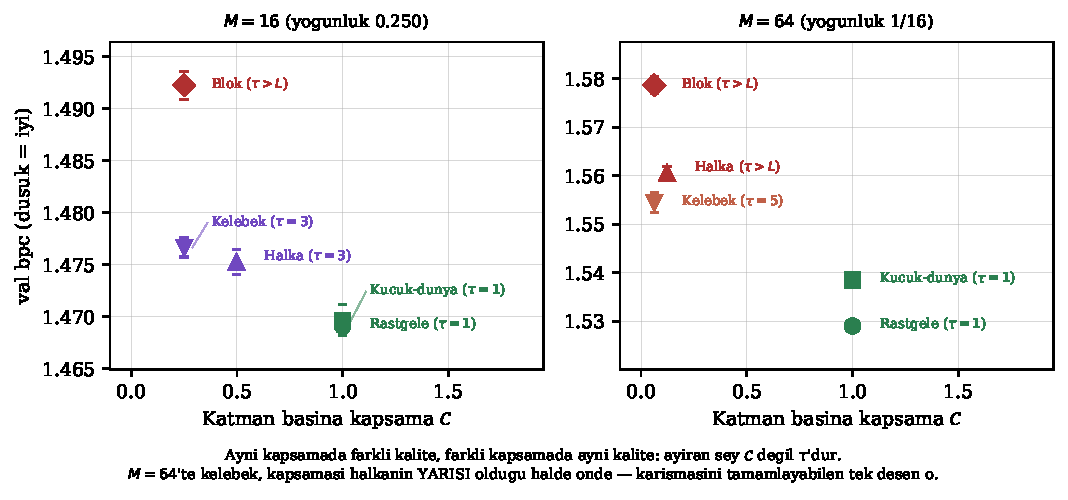
\includegraphics[width=0.92\textwidth]{fig_tau.pdf}
\caption{Kaliteyi ayıran şey katman başına kapsama değil karışma derinliğidir. Yatay eksen
$\mathcal{C}$, dikey eksen val bpc; renk $\tau$'yu gösterir. Solda ($M{=}16$) kelebek ile blok
aynı $\mathcal{C}$'ye sahiptir ama $9.6\sigma$ ayrışır, halka ile kelebek iki kat farklı
$\mathcal{C}$'ye sahiptir ama ayırt edilemez. Sağda ($M{=}64$) iki ölçü \emph{sırada}
çelişir: kelebeğin kapsaması halkanın yarısıdır, yine de öndedir --- karışmasını
tamamlayabilen tek desen odur.}
\label{fig:tau}
\end{figure*}

\begin{table*}[!t]
\centering
\footnotesize
\caption{Kalite: yoğunluk taraması ($L{=}8$, \texttt{mixed}, karakter düzeyi \texttt{text8},
bpc). $\sigma$: farkın yoğun modele göre standart hataya oranı; $\sigma<2$ gürültü. $n$: tohum.}
\label{tab:kalite}
\begin{tabular}{@{}llccccc@{}}
\toprule
Desen & $M$ & Yoğunluk & Kapsama & val bpc & Yoğun'a fark & $\sigma$ \\
\midrule
Yoğun          & 8  & 0.500 & 1.000 & 1.4466 & ---       & ---  \\
Halka          & 8  & 0.500 & 0.998 & 1.4467 & $+0.0001$ & 0.1  \\
Rastgele       & 8  & 0.500 & 1.000 & 1.4467 & $+0.0001$ & 0.0  \\
Küçük-dünya    & 8  & 0.500 & 1.000 & 1.4485 & $+0.0019$ & 1.2  \\
Blok           & 8  & 0.500 & 0.500 & 1.4527 & $+0.0061$ & 3.5  \\
Mozaik         & 8  & 0.500 & 0.500 & 1.4541 & $+0.0075$ & 3.9  \\
\midrule
Rastgele       & 16 & 0.250 & 1.000 & 1.4682 & $+0.0216$ & 16.4 \\
Küçük-dünya    & 16 & 0.250 & 1.000 & 1.4696 & $+0.0230$ & 13.3 \\
Halka          & 16 & 0.250 & 0.498 & 1.4752 & $+0.0286$ & 19.4 \\
Kelebek        & 16 & 0.250 & 0.250 & 1.4765 & $+0.0299$ & 14.2 \\
Blok           & 16 & 0.250 & 0.250 & 1.4923 & $+0.0457$ & 28.4 \\
Mozaik         & 16 & 0.250 & 0.250 & 1.4925 & $+0.0459$ & 18.4 \\
\midrule
Rastgele       & 32 & 0.125 & 1.000 & 1.5034 & $+0.0568$ & 28.2 \\
Küçük-dünya    & 32 & 0.125 & 1.000 & 1.5072 & $+0.0606$ & 40.4 \\
Kelebek        & 32 & 0.125 & 0.125 & 1.5197 & $+0.0731$ & 20.3 \\
Halka          & 32 & 0.125 & 0.248 & 1.5208 & $+0.0742$ & 58.9 \\
Blok           & 32 & 0.125 & 0.125 & 1.5488 & $+0.1022$ & 44.2 \\
\midrule
Rastgele       & 64 & 0.062 & 1.000 & 1.5290 & $+0.0824$ & 61.3 \\
Küçük-dünya    & 64 & 0.062 & 1.000 & 1.5385 & $+0.0919$ & 88.7 \\
Kelebek        & 64 & 0.062 & 0.062 & 1.5544 & $+0.1078$ & 48.1 \\
Halka          & 64 & 0.062 & 0.123 & 1.5606 & $+0.1140$ & 72.5 \\
Blok           & 64 & 0.062 & 0.062 & 1.5787 & $+0.1321$ & 68.2 \\
\bottomrule
\end{tabular}
\end{table*}

\subsection{Derinlik: $\tau$ ile $L$'nin etkileşimi}
Tablo~\ref{tab:derinlik}, halka ile rastgele arasındaki farkın ağ derinliğiyle nasıl
değiştiğini gösterir. Fark tek yönlü büyümez; $2.8\sigma \to 0.3\sigma \to 4.3\sigma \to
23.3\sigma$ seyri izler (Şekil~\ref{fig:derinlik}). Bu tek-tepeli olmayan seyir, $\tau$ ile
$L$'nin karşılaştırılmasıyla açıklanır ve üç rejim ortaya çıkarır.

$L<\tau$ rejiminde ($L{=}2$) halka karışmasını tamamlayamaz ve ceza öder. $L\approx\tau$
rejiminde ($L{=}4$, halka için $\tau{=}3$) karışma tam olarak biter ve açık \emph{kapanır}
($0.3\sigma$; işaret bile terse döner, yani fark tümüyle gürültüye iner); bu, derinliğin
zayıf karışımı gerçekten kurtardığı tek noktadır. $L>\tau$
rejiminde ($L{=}8,16$) açık yeniden büyür, çünkü artık sınırlayıcı olan kapsama değil
\emph{doygunluktur}: sabit bir desen $\tau$'dan sonraki katmanlarda yeni bağlantı eklemez,
oysa katmandan katmana değişen bir desen her katmanda yeni bir karıştırma uygular. Böylece
derinlik bulgusu tek bir etki değil, iki farklı mekanizmanın ($\tau$ eşiği ve doygunluk)
kesişimidir. İkinci mekanizma ShuffleSparse \cite{shufflesparse2025} teorisinin
öngördüğüdür ve onu bağımsız ölçümle doğrular.

$\tau$ bu satırların tümünü sıralamaz. $L{=}2$'de tüm seyrek varyantlar yoğun modeli geniş
bir farkla ($\sim\!0.07$ bpc) geçer: sığ ağda eşit-parametre protokolünün genişlettiği gizli
katman, topoloji farklarını bastırır. O satırda desenler arası yayılım $0.009$ bpc'ye iner
ve kelebek --- birikmiş kapsaması en düşük varyant --- nominal olarak en iyi çıkar. Yani
karışma derinliği sığ rejimde açıklayıcı değildir; genişlik baskındır.

\begin{figure}[!t]
\centering
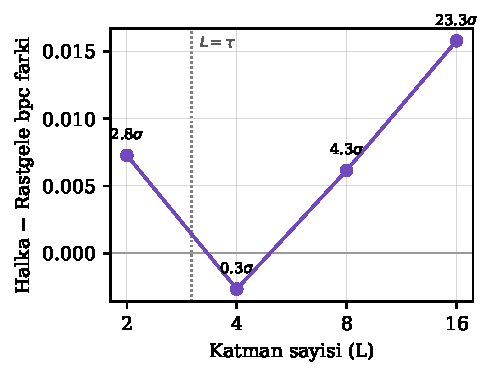
\includegraphics[width=0.95\columnwidth]{fig_derinlik.pdf}
\caption{Halka ile rastgele arasındaki bpc farkının derinlikle değişimi ($M{=}16$). Fark
$L{=}16$'da $20.3\sigma$'ya ulaşır; sabit desen (halka) derinlikten faydalanamadığı için
makas açılır. Etiketler istatistiksel anlamlılığı ($\sigma$) gösterir.}
\label{fig:derinlik}
\end{figure}

\begin{table}[!t]
\centering
\footnotesize
\caption{Derinlik: halka$-$rastgele farkı tek yönlü büyümez, $\tau$ eşiğinde kapanır
($M{=}16$, \texttt{mixed}). Halka için $\tau{=}3$; açık yalnızca $L{\approx}\tau$ olduğunda
yok olur, $L>\tau$ olduğunda doygunluk nedeniyle yeniden açılır.}
\label{tab:derinlik}
\begin{tabular}{@{}lcccccc@{}}
\toprule
$L$ & Rejim & Yoğun & Rast. & Halka & Kelebek & H$-$R ($\sigma$) \\
\midrule
2  & $L<\tau$      & 1.6338 & 1.5664 & 1.5736 & 1.5650 & $+0.0073$ (2.8) \\
4  & $L\approx\tau$& 1.5285 & 1.5454 & 1.5428 & 1.5420 & $-0.0027$ (0.3) \\
8  & $L>\tau$      & 1.4466 & 1.4691 & 1.4752 & 1.4766 & $+0.0062$ (4.3) \\
16 & $L>\tau$      & 1.4024 & 1.4364 & 1.4521 & 1.4463 & $+0.0158$ (23.3) \\
\bottomrule
\end{tabular}
\end{table}

\subsection{Sabit-maske kontrolü: iki bulgunun ayrıştırılması}
\label{sec:sabit}
Yukarıdaki iki bulgu --- ``yapısız rastgele en iyidir'' ve ``derinlikle değişen desenler
avantajlıdır'' --- ilk kurulumumuzda ayrışmıyordu. Uygulamamız varyans azaltmak için her
katmana farklı bir maske tohumu veriyor; yan etkisi olarak tohum tüketen desenler (rastgele,
küçük-dünya) katmandan katmana \emph{yeniden çizilir}, kelebek de aşamasıyla zaten öyledir.
Dolayısıyla rastgele kontrol grubunun kendisi derinlikle değişen bir desendi.

Bunu ayırmak için topolojiyi tüm katmanlarda sabitleyen, ancak tohumlar arasında değiştirmeye
devam eden bir kontrol koştuk (böylece varyans azaltma korunur, yalnızca derinlik ekseni
kapanır). Denklem~\eqref{eq:tau} bu kontrol için iki \emph{çürütülebilir} öngörü verir ve
öngörüleri koşulardan önce kaydettik: (i) sabit rastgelenin $\tau$'su da $1$ olduğundan
kalitesi \emph{değişmemeli}; (ii) aşaması dondurulan kelebeğin $\tau$'su $>L$'ye çıktığından
bloğun seviyesine \emph{düşmeli}. Ayrıca halka için bayrak tanımı gereği etkisizdir; bunu boş
kontrol olarak kullandık. Sonuçlar Tablo~\ref{tab:sabit}'te.

Boş kontrol geçti: halkada sabit ile değişken arasındaki fark $0.49\sigma$; aynı tohumda
eşleştirildiğinde ortalama mutlak fark $0.0012$ bpc, yani tohumlar arası standart sapmanın
($0.0033$) üçte biri ve işareti tohumdan tohuma değişiyor --- bu, TF32 ve atomik indirgeme
kaynaklı koşu-içi belirsizliktir, sistematik bir etki değil.

Birinci öngörü doğrulandı: sabit rastgele üç derinlikte de değişkeninden ayırt edilemedi
($0.88\sigma$, $0.48\sigma$, $1.26\sigma$). Yani ``yapısız rastgele en iyidir'' bulgusu bir
kapsama etkisidir, katmanlar arası yeniden çizimin eseri değildir; iki bulgu bağımsızdır.

İkinci öngörü nicel olarak doğrulandı ve $\tau$'nun en güçlü kanıtıdır. Aşaması dondurulan
kelebek $L{=}8$'de $1.4766$'dan $1.4927$'ye düşer ($5.4\sigma$) --- ve bu değer, aynı
kapsamaya sahip bloğun $1.4923$'ünden $0.14\sigma$ uzaktadır. Yani $\tau$ yalnızca bir yön
değil, bir \emph{nokta} öngörmüş ve tutturmuştur: kelebeği bloktan ayıran şey bağlantı
sayısı veya katman içi kapsaması değil, yalnızca aşamasının katmandan katmana dönmesidir.
Etki derinlikle büyür ($+0.0064 \to +0.0161 \to +0.0373$), ki bu da doygunluk mekanizmasının
beklentisidir: sabit desen $\tau$'dan sonraki her katmanı boşa harcar. $L{=}4$'te fark doğru
yöndedir fakat anlamlı değildir ($1.08\sigma$); o derinlikte desenler arası toplam yayılım
zaten $0.02$ bpc mertebesindedir.

\begin{table}[!t]
\centering
\footnotesize
\caption{Sabit-maske kontrolü ($M{=}16$). Topoloji tüm katmanlarda sabitlenir, tohumlar arası
değişmeye devam eder. Öngörüler koşulardan önce kaydedilmiştir.}
\label{tab:sabit}
\begin{tabular}{@{}llccc@{}}
\toprule
Desen & $L$ & Değişken & Sabit & $\Delta$ ($\sigma$) \\
\midrule
\multicolumn{5}{@{}l}{\emph{Boş kontrol} --- öngörü: etkisiz} \\
Halka     & 8  & 1.4752 & 1.4764 & $+0.0011$ (0.5) \\
\midrule
\multicolumn{5}{@{}l}{\emph{Ana kontrol} --- öngörü: değişmemeli ($\tau{=}1 \to 1$)} \\
Rastgele  & 4  & 1.5454 & 1.5508 & $+0.0054$ (0.9) \\
Rastgele  & 8  & 1.4691 & 1.4698 & $+0.0008$ (0.5) \\
Rastgele  & 16 & 1.4364 & 1.4346 & $-0.0017$ (1.3) \\
\midrule
\multicolumn{5}{@{}l}{\emph{Keskin test} --- öngörü: bloğa düşmeli ($\tau{=}3 \to {>}L$)} \\
Kelebek   & 4  & 1.5420 & 1.5484 & $+0.0064$ (1.1) \\
Kelebek   & 8  & 1.4766 & \textbf{1.4927} & $+0.0161$ (5.4) \\
Kelebek   & 16 & 1.4463 & 1.4836 & $+0.0373$ (28.9) \\
\midrule
\multicolumn{5}{@{}l}{Blok ($L{=}8$, aynı $\mathcal{C}{=}0.250$): $1.4923$ ---
sabit kelebeğe $0.14\sigma$} \\
\bottomrule
\end{tabular}
\end{table}

\subsection{Kontrol deneyleri}
\emph{Başlangıç ölçeği.} Seyrek katmanların GELU'ya farklı ölçekte sinyal soktuğunu gözlemledik
(çıkış std'si $1.41$ vs $0.45$). Tüm ana bulguları üç başlangıç rejiminde tekrarladık; kapsama
sıralaması üçünde de korundu, yani sonuçlar başlangıç seçiminden bağımsızdır.

\emph{Öz-rehberli eğitim.} Kazanç bir faz geçişi gösterir (Tablo~\ref{tab:kilavuz}): $L\le 8$'de
hiçbir desende anlamlı etki yokken, $L{=}16$'da üç desende birden anlamlı iyileşme belirir.
Kılavuzsuz derin modeller kilitlenmedi; kazanç bir ``kurtarma'' değil $\sim\!1\%$'lik bir
iyileşmedir. Kritik olarak, kılavuz altında kelebeğin halkaya görünür üstünlüğü kaybolur
($12.0\sigma \to 1.5\sigma$); bu, ``derinlikle değişen desen daha iyi kalite verir'' naif
yorumunun büyük ölçüde bir optimizasyon eseri olduğunu gösterir. Doğru ifade: kelebek, halkayla
\emph{aynı} kaliteyi yarı iletişimle verir.

\begin{table}[!t]
\centering
\footnotesize
\caption{Öz-rehberli eğitimin derinliğe göre etkisi ($M{=}16$). Faz geçişi: $L\le8$ etkisiz,
$L{=}16$ anlamlı.}
\label{tab:kilavuz}
\begin{tabular}{@{}llccc@{}}
\toprule
$L$ & Desen & Kılavuzsuz & Kılavuzlu & Kazanç ($\sigma$) \\
\midrule
8  & Kelebek  & 1.4765 & 1.4727 & $+0.0038$ (1.8) \\
8  & Rastgele & 1.4682 & 1.4696 & $-0.0014$ (0.9) \\
8  & Halka    & 1.4752 & 1.4724 & $+0.0028$ (1.5) \\
16 & Kelebek  & 1.4457 & 1.4339 & $+0.0118$ (13.5) \\
16 & Rastgele & 1.4373 & 1.4273 & $+0.0099$ (4.9)  \\
16 & Halka    & 1.4521 & 1.4363 & $+0.0158$ (10.6) \\
\bottomrule
\end{tabular}
\end{table}

\subsection{Dağıtık iletişim}
Tablo~\ref{tab:dagitik}, dört parçalama stratejisinin sekiz H200 üzerinde, rank başına eşit
parametreyle ölçülen değerlerini gösterir. Kelebek parçalama muhatap sayısını $7$'den $1$'e,
FFN iletişim hacmini $\sim\!7\times$ düşürür ve ileri geçişte halka ve yoğun TP'den hızlıdır.
\emph{Kritik uyarı:} bu $7\times$ yalnızca FFN'e aittir; dikkat katmanı da her iki stratejide
all-reduce gerektirdiğinden uçtan uca iletişim azalması $\sim\!2\times$ ile sınırlıdır. Ayrı
bir deneyde dikkatsiz bir FFN yığınını sekiz H200 üzerinde uçtan uca eğittik; rank başına
parametre eşit tutulduğunda geniş-seyrek varyantlar (halka $2.02$, kelebek $2.04$ bpc)
dar-yoğun tensor-paralelden ($2.73$) belirgin biçimde iyidir; bu, dağıtık parçalamanın
gerçekten eğitilebilir olduğunu doğrular.

\begin{table}[!t]
\centering
\footnotesize
\caption{Dağıtık iletişim ($8{\times}$H200, $d{=}8192$, rank başına eşit parametre).}
\label{tab:dagitik}
\begin{tabular}{@{}lccc@{}}
\toprule
Parçalama & İletişim (MB/adım) & Muhatap & İleri (ms) \\
\midrule
Yoğun tensor-paralel & 469.8 & 7 & 4.25 \\
Halka                & 134.2 & 2 & 2.83 \\
Kelebek              & 67.1  & 1 & 2.51 \\
Blok                 & 0.0   & 0 & 1.90 \\
\bottomrule
\end{tabular}
\end{table}

\subsection{Uygulama ve ölçekleme}
Kelebeğin bmm uygulamasının maskeliyle aynı kaliteyi verdiğini doğruladık (fark $\le 0.0007$
bpc), ancak bmm bu ölçekte $\sim\!1.9\times$ \emph{yavaştır}: XOR eşleşmesi için gereken
toplama/birleştirme adımları bellek-bağımlıdır. Bu uygulamaya özgüdür; Monarch \cite{dao2022}
füzyonlu bir çekirdekle aynı yapıda $2\times$ hızlanma gösterir. Ölçeklemede ($\sim\!403$M,
Tablo~\ref{tab:olcek}) yoğun modelin $0.91$ bpc'si güçlü tabanların mertebesindedir.
Ortalamaların sıralaması küçük ölçektekiyle aynıdır (yoğun $\le$ rastgele $\le$ kelebek),
ancak kendi $\sigma\!\ge\!2$ ölçütümüzü bu tabloya uyguladığımızda tabloyu olduğu gibi
raporlamak gerekir: yoğun ile rastgele arasındaki fark bu ölçekte \emph{anlamlı değildir}
($+0.0097$ bpc, $1.34\sigma$, $n{=}2$), yoğun ile kelebek de sınırdadır ($1.95\sigma$); yoğun
modelin iki tohum arası saçılımı ($\pm0.0101$) farkın kendisinden büyüktür. Anlamlı kalan tek
karşılaştırma rastgele ile kelebek arasındadır ($+0.0043$ bpc, $5.36\sigma$) ve bu açık küçük
ölçeğe göre yarıya iner ($12.5\sigma \to 5.4\sigma$) fakat kapanmaz. Dolayısıyla bu deneyin
desteklediği ifade ``seyrekliğin kalite bedeli 403M'de sürüyor'' değil, ``o bedel bu bütçede
ölçüm gürültüsüne gömülmüştür''dir; iki tohum daha güçlü bir hüküm için yetersizdir.

\begin{table}[!t]
\centering
\footnotesize
\caption{Ölçekleme: $\sim\!403$M ($d{=}1024$, $L{=}32$, bayt düzeyi \texttt{enwik9}, 2 tohum).
Bellek/hız maskeli uygulamaya aittir.}
\label{tab:olcek}
\begin{tabular}{@{}lcccc@{}}
\toprule
Desen & val bpc & $\pm$ & Bellek (GB) & bin tok/s \\
\midrule
Yoğun    & 0.9096 & 0.0101 & 38 & 771 \\
Rastgele & 0.9193 & 0.0011 & 99 & 329 \\
Kelebek  & 0.9236 & 0.0003 & 99 & 337 \\
\bottomrule
\end{tabular}
\end{table}

% ============================================================
\section{Bilgi-Teorik Sınır}
\label{sec:sinir-teori}
% ============================================================
$P$ dilime bölünmüş bir FFN katmanında, bir dilim başka $k$ dilimle haberleşiyorsa, o katmanda
hesaplayabildiği çıktı birimleri en fazla girdilerin $(k{+}1)/P$ oranına bağlı olabilir.
Dolayısıyla katman başına kapsama
\begin{equation}
\mathcal{C}_{\text{katman}} \le \frac{k+1}{P}
\end{equation}
ile sınırlıdır. Tam kapsama ($\mathcal{C}_{\text{katman}}{=}1$) ancak $k{=}P{-}1$ (all-to-all)
ile mümkündür. Buradan bir imkânsızlık çıkar: katman başına tam kapsama ile tek-muhatap ($k{=}1$)
iletişim aynı katmanda bağdaşmaz. Tek-muhatapla tam karışım ancak derinlikte kazanılır: kelebek
her katmanda farklı bir eşle ($r\oplus 2^\ell$) haberleşerek $\log_2(P)$ katmanda tam karışıma
ulaşır; sabit komşulu halka $P/2$ katman gerektirir. Kapsamayı derinlikte geri kazanmanın küçük
ama kalıcı bir kalite bedeli vardır (ölçtüğümüz kelebek--rastgele açığı ölçekle incelir fakat
kapanmaz). Bu bir mühendislik eksiği değil, tasarım uzayını sınırlayan bir yasadır.

% ============================================================
\section{Karar Modeli}
% ============================================================
Kelebek parçalama üç koşul birden sağlandığında rasyoneldir: (i) model tek veri merkezine
sığmayacak kadar büyük; (ii) merkezler-arası hat yoğun TP'ye yetmeyecek kadar dar; (iii) ama
kelebeğe yetecek kadar hızlı. Ölçülen iletişim değerlerini kullanan model, bu koridorun
pratikte $\sim\!400$ Gbps üstü (aynı şehir/dedike fiber) hatlar için açıldığını, tüketici
internetinde ise kelebeğin bile yetersiz kaldığını gösterir (Tablo~\ref{tab:karar}). Büyük
resimde, merkezler-arası katman-katman parçalama neredeyse her durumda kötü bir fikirdir;
kelebeğin gerçek yeri çok sayıda düğümün hızlı bir dokuyla bağlandığı merkez-içi büyük
kümelerdir.

\begin{table}[!t]
\centering
\footnotesize
\caption{Karar modeli örnekleri. Kelebek yalnızca dar bir koridorda rasyoneldir.}
\label{tab:karar}
\begin{tabular}{@{}p{3.2cm}p{1.6cm}p{2.4cm}@{}}
\toprule
Senaryo & Rejim & Karar \\
\midrule
7B, tek merkeze sığar    & ---          & Bölme; veri-paralel \\
500B, 400 Gbps dedike    & koridor      & \textbf{Kelebeği kullan} \\
500B, 100 Gbps           & hat-bağımlı  & Kelebek de yetmez \\
500B, tüketici interneti & hat-bağımlı  & Model-paralel deneme \\
\bottomrule
\end{tabular}
\end{table}

% ============================================================
\section{Sınırlar}
\label{sec:sinir}
% ============================================================
(1) Yalnızca FFN parçalandı; dikkat de all-reduce gerektirdiğinden uçtan uca kazanç
$\sim\!2\times$ ile sınırlıdır. (2) bmm uygulaması naiftir; füzyonlu bir çekirdek durumu
tersine çevirebilir. (3) Kalite deneylerindeki bellek maliyeti, adil karşılaştırma için gizli
katmanı genişletme tercihimizin sonucudur; parçalanmış bir uygulamada oluşmaz. (4) Gerçek bir
geniş alan ağı üzerinde uçtan uca eğitim yapılmadı; karar modeli yalnızca bant genişliğine
dayanır, gecikme ve kayıp içermez. (5) Optimizasyon zorluğunun mekanizması ölçülmedi,
yalnızca sonucu gözlendi. (6) Katman başına kapsama tek başına yetersizdir (eşit kapsamada
$6.7\sigma$ fark); karışma derinliği $\tau$ bu karşıörnekleri çözer, fakat sıralayıcı bir
ölçüdür: küçük $\tau$ farkları düşük seyreklikte gürültünün altında kalır ve sığ ağda
($L{=}2$) genişlik etkisi baskın olduğu için hiç açıklayıcı değildir.

(7) $\tau$, sabit-maske kontrolünde (Bölüm~\ref{sec:sabit}) iki öngörüsünü de tutturmuştur;
ancak $M{=}16$, $L\in\{4,8,16\}$ ile sınırlı kalmıştır. Diğer yoğunluklarda ve küçük-dünya
gibi tohum tüketen öteki desenlerde tekrarlanmamıştır. Ayrıca $\tau$ ikili bir erişilebilirlik
ölçüsüdür ve erişimin dağılımını görmez; en seyrek rejimde ($M{=}64$) aynı $\tau$'ya sahip iki
deseni ayırt edemediği bir durum ölçtük ($8.2\sigma$).

(8) Deneyler karakter düzeyinde \texttt{text8} ve bayt düzeyinde \texttt{enwik9} üzerindedir;
alt-kelime (BPE) sözlüğü kullanan modellerde FFN'in karıştırma yükü farklı olabileceğinden
bulguların o rejime taşınması doğrulanmamıştır.

% ============================================================
\section{Sonuç}
% ============================================================
Bu çalışma bir yöntem önermiyor, bir ödünleşimi haritalıyor. Yoğun FFN matrisi varsayımını
terk etmenin tek bir hızlandırıcıda kalite kazandırmadığını; yoğunluk $1/2$'ye kadar
bedelsiz, ötesinde maliyetli olduğunu; yapısız rastgele seyrekliğin her yapılandırılmış desenden
iyi olduğunu gösterdik. Hız tarafında ölçtüğümüz şey daha dardır: \emph{bizim} maskeli ve bmm
uygulamalarımız hızlanma üretmemiştir ve bunun nedenini bellek-bağımlı toplama/birleştirme
adımlarına bağlıyoruz; füzyonlu bir çekirdeğin durumu tersine çevirebileceğini
\cite{dao2022} göz önünde tutarak ``yapısal seyreklik hızlanma vermez'' gibi genel bir
sonuç çıkarmıyoruz. Kaliteyi belirleyenin katman başına kapsama değil karışma derinliği
olduğunu, derinliğin etkisinin $\tau$ eşiğine göre yön değiştirdiğini ölçtük. Kazancın
yalnızca dağıtık iletişimde --- kelebeğin halkayla aynı
kaliteyi yarı iletişim ve tek muhatapla verdiğinde --- ortaya çıktığını, fakat bunun bir
bilgi-teorik sınıra ve küçük kalıcı bir kalite bedeline tabi olduğunu belirledik. Başlangıç
motivasyonu olan ``dağınık kaynakları internet üzerinden birleştirme'' hedefinin ağırlık
yapısını değiştirmekle çözülmediğini gösterdik. Çalışmanın katkısı, iletişim ile kalite
arasındaki temel takasın nerede durduğunu kontrollü biçimde haritalamaktır: sonuç bir reçete
değil, bir pusuladır.

\emph{Yeniden üretilebilirlik.} Tüm deneyler (326 koşu) çoklu tohumla tekrarlanmış; kod, SLURM
betikleri ve ham sonuç dosyaları açık biçimde saklanmaktadır.

% ============================================================
\section*{Teşekkür}
% ============================================================
Bu araştırmada yer alan tüm nümerik hesaplamalar TÜBİTAK ULAKBİM, Yüksek Başarım ve Grid
Hesaplama Merkezi'nde (TRUBA kaynaklarında) gerçekleştirilmiştir.

% ============================================================
% IEEE stili kaynakca
% ============================================================
\begin{thebibliography}{1}
\bibitem{wei2024}
X. Wei, S. Moalla, R. Pascanu, and C. Gülçehre, ``Building on efficient foundations:
Effectively training LLMs with structured feedforward layers,'' in \emph{Proc. Adv. Neural
Inf. Process. Syst. (NeurIPS)}, 2024.

\bibitem{dao2022}
T. Dao \emph{et al.}, ``Monarch: Expressive structured matrices for efficient and accurate
training,'' in \emph{Proc. Int. Conf. Mach. Learn. (ICML)}, 2022. [Online]. Available:
arXiv:2204.00595.

\bibitem{vaswani2017}
A. Vaswani \emph{et al.}, ``Attention is all you need,'' in \emph{Proc. Adv. Neural Inf.
Process. Syst. (NeurIPS)}, 2017, pp.~5998--6008.

\bibitem{kaplan2020}
J. Kaplan \emph{et al.}, ``Scaling laws for neural language models,'' 2020. [Online].
Available: arXiv:2001.08361.

\bibitem{chinchilla2022}
J. Hoffmann \emph{et al.}, ``Training compute-optimal large language models,'' in
\emph{Proc. Adv. Neural Inf. Process. Syst. (NeurIPS)}, 2022.

\bibitem{megatron2019}
M. Shoeybi, M. Patwary, R. Puri, P. LeGresley, J. Casper, and B. Catanzaro, ``Megatron-LM:
Training multi-billion parameter language models using model parallelism,'' 2019. [Online].
Available: arXiv:1909.08053.

\bibitem{narayanan2021}
D. Narayanan \emph{et al.}, ``Efficient large-scale language model training on GPU clusters
using Megatron-LM,'' in \emph{Proc. Int. Conf. High Perform. Comput., Netw., Storage Anal.
(SC)}, 2021.

\bibitem{zero2020}
S. Rajbhandari, J. Rasley, O. Ruwase, and Y. He, ``ZeRO: Memory optimizations toward training
trillion parameter models,'' in \emph{Proc. Int. Conf. High Perform. Comput., Netw., Storage
Anal. (SC)}, 2020.

\bibitem{fsdp2023}
Y. Zhao \emph{et al.}, ``PyTorch FSDP: Experiences on scaling fully sharded data parallel,''
\emph{Proc. VLDB Endow.}, vol.~16, no.~12, pp.~3848--3860, 2023.

\bibitem{gpipe2019}
Y. Huang \emph{et al.}, ``GPipe: Efficient training of giant neural networks using pipeline
parallelism,'' in \emph{Proc. Adv. Neural Inf. Process. Syst. (NeurIPS)}, 2019.

\bibitem{korthikanti2023}
V. Korthikanti \emph{et al.}, ``Reducing activation recomputation in large transformer
models,'' in \emph{Proc. Mach. Learn. Syst. (MLSys)}, 2023.

\bibitem{ringattn2023}
H. Liu, M. Zaharia, and P. Abbeel, ``Ring attention with blockwise transformers for
near-infinite context,'' 2023. [Online]. Available: arXiv:2310.01889.

\bibitem{han2015}
S. Han, J. Pool, J. Tran, and W. Dally, ``Learning both weights and connections for efficient
neural networks,'' in \emph{Proc. Adv. Neural Inf. Process. Syst. (NeurIPS)}, 2015.

\bibitem{frankle2019}
J. Frankle and M. Carbin, ``The lottery ticket hypothesis: Finding sparse, trainable neural
networks,'' in \emph{Proc. Int. Conf. Learn. Represent. (ICLR)}, 2019.

\bibitem{rigl2020}
U. Evci, T. Gale, J. Menick, P. S. Castro, and E. Elsen, ``Rigging the lottery: Making all
tickets winners,'' in \emph{Proc. Int. Conf. Mach. Learn. (ICML)}, 2020.

\bibitem{sparsegpt2023}
E. Frantar and D. Alistarh, ``SparseGPT: Massive language models can be accurately pruned in
one-shot,'' in \emph{Proc. Int. Conf. Mach. Learn. (ICML)}, 2023.

\bibitem{nm2021}
A. Mishra \emph{et al.}, ``Accelerating sparse deep neural networks,'' 2021. [Online].
Available: arXiv:2104.08378.

\bibitem{expander2018}
A. Prabhu, G. Varma, and A. Namboodiri, ``Deep expander networks: Efficient deep networks from
graph theory,'' in \emph{Proc. Eur. Conf. Comput. Vis. (ECCV)}, 2018.

\bibitem{dao2019}
T. Dao, A. Gu, M. Eichhorn, A. Rudra, and C. Ré, ``Learning fast algorithms for linear
transforms using butterfly factorizations,'' in \emph{Proc. Int. Conf. Mach. Learn. (ICML)},
2019.

\bibitem{pixelbutterfly2022}
B. Chen, T. Dao, K. Liang, J. Yang, Z. Song, A. Rudra, and C. Ré, ``Pixelated butterfly:
Simple and efficient sparse training for neural network models,'' in \emph{Proc. Int. Conf.
Learn. Represent. (ICLR)}, 2022.

\bibitem{shazeer2017}
N. Shazeer \emph{et al.}, ``Outrageously large neural networks: The sparsely-gated
mixture-of-experts layer,'' in \emph{Proc. Int. Conf. Learn. Represent. (ICLR)}, 2017.

\bibitem{gshard2021}
D. Lepikhin \emph{et al.}, ``GShard: Scaling giant models with conditional computation and
automatic sharding,'' in \emph{Proc. Int. Conf. Learn. Represent. (ICLR)}, 2021.

\bibitem{stich2019}
S. U. Stich, ``Local SGD converges fast and communicates little,'' in \emph{Proc. Int. Conf.
Learn. Represent. (ICLR)}, 2019.

\bibitem{swarm2023}
M. Ryabinin, T. Dettmers, M. Diskin, and A. Borzunov, ``SWARM parallelism: Training large
models can be surprisingly communication-efficient,'' in \emph{Proc. Int. Conf. Mach. Learn.
(ICML)}, 2023.

\bibitem{petals2023}
A. Borzunov \emph{et al.}, ``Petals: Collaborative inference and fine-tuning of large models,''
in \emph{Proc. Assoc. Comput. Linguistics (ACL), System Demonstrations}, 2023.

\bibitem{mahoney2011}
M. Mahoney, ``Large text compression benchmark,'' 2011. [Online]. Available:
http://mattmahoney.net/dc/text.html.

\bibitem{switch2022}
W. Fedus, B. Zoph, and N. Shazeer, ``Switch Transformer: Scaling to trillion parameter models
with simple and efficient sparsity,'' \emph{J. Mach. Learn. Res.}, vol.~23, no.~120,
pp.~1--39, 2022.

\bibitem{diloco2023}
A. Douillard \emph{et al.}, ``DiLoCo: Distributed low-communication training of language
models,'' 2023. [Online]. Available: arXiv:2311.08105.

\bibitem{shufflesparse2025}
A. Tyagi \emph{et al.}, ``ShuffleSparse: Learned shuffles for structured sparse networks,''
2025. [Online]. Available: arXiv:2510.14812.

\bibitem{bdlora2025}
``Block-diagonal LoRA for eliminating communication overhead in tensor parallel LoRA
serving,'' 2025. [Online]. Available: arXiv:2510.23346.

\bibitem{detransformer2024}
``Communication-efficient model parallelism for distributed in-situ transformer inference,''
in \emph{Proc. Design, Automation Test Eur. Conf. (DATE)}, 2024.

\bibitem{flashcomm2024}
``Flash communication: Reducing tensor parallelization bottleneck for fast LLM inference,''
2024. [Online]. Available: arXiv:2412.04964.
\end{thebibliography}

\end{document}
